\documentclass[12pt]{article}

\usepackage{a4wide,graphicx,amsmath,amssymb,amsfonts,url,psfrag,subcaption}
\usepackage{rotating}
\usepackage{xcolor}
\usepackage{soul}
\usepackage{tikz}
\usepackage{algorithm2e}
\usepackage{todonotes}

\addtolength{\parskip}{3mm}

\usepackage[numbers,sort&compress]{natbib}
\usepackage{lineno, blindtext}
\usepackage[export]{adjustbox}

%\usepackage[dvipsnames]{xcolor}
\definecolor{MyGreen}{HTML}{66C2A5}
\definecolor{MyOrange}{HTML}{FC8D62}
\definecolor{MyBlue}{HTML}{8DA0CB}
\definecolor{MyPink}{HTML}{E78AC3}
\definecolor{MyGreen2}{HTML}{A6D854}
% Notes
\newcommand{\notes}[1]{\textit{\bf[***note -- #1***]}}
\begin{document}



%%%%%%% Figure %%%%%%%%
\begin{figure}[h]
%
\vspace{-0.5cm}
\begin{center}
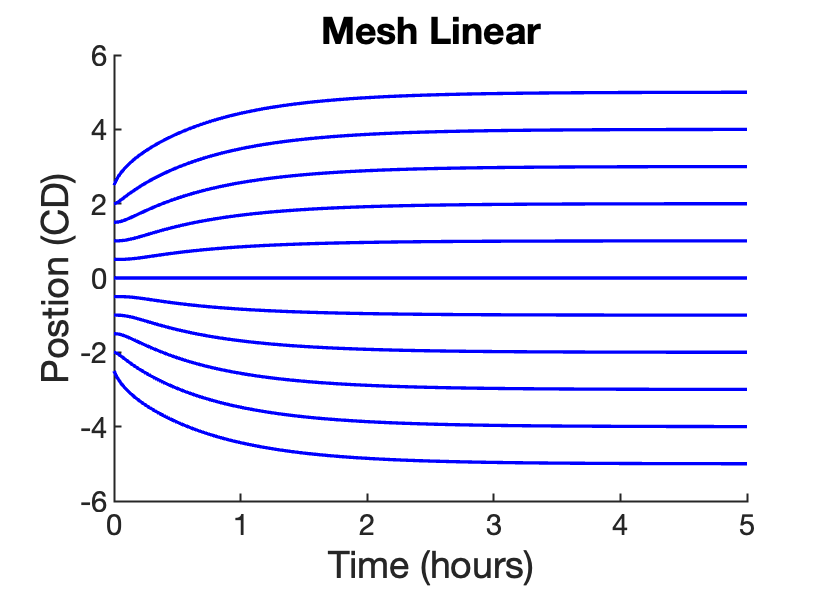
\includegraphics[width=4.9cm, trim={0.0cm 0.0cm 0.0cm 0.0cm}, clip]{Figs/Test02aMonolayerGrowth1dChainHomogeneousChainMesh_Linear.png}
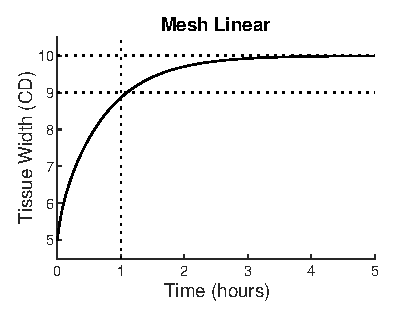
\includegraphics[width=4.9cm, trim={0.0cm 0.0cm 0.0cm 0.0cm}, clip]{Figs/Test02aMonolayerGrowth1dChainHomogeneousChainMesh_LinearWidth}
\end{center}
\vspace{-0.5cm}
\caption{{\bf VT homogeneous.} 
	TODO. }
\label{fig:todo}
\end{figure}

%%%%%%% Figure %%%%%%%%
\begin{figure}[h]
%
\begin{center}
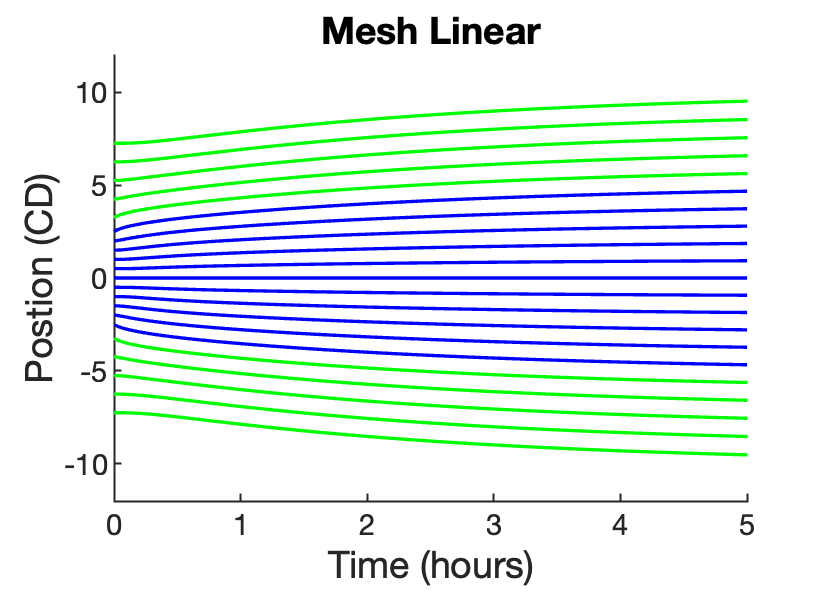
\includegraphics[width=4.9cm, trim={0.0cm 0.0cm 0.0cm 0.0cm}, clip]{Figs/Test02aMonolayerGrowth1dChainHeterogeneousChainMesh_Linear.png}
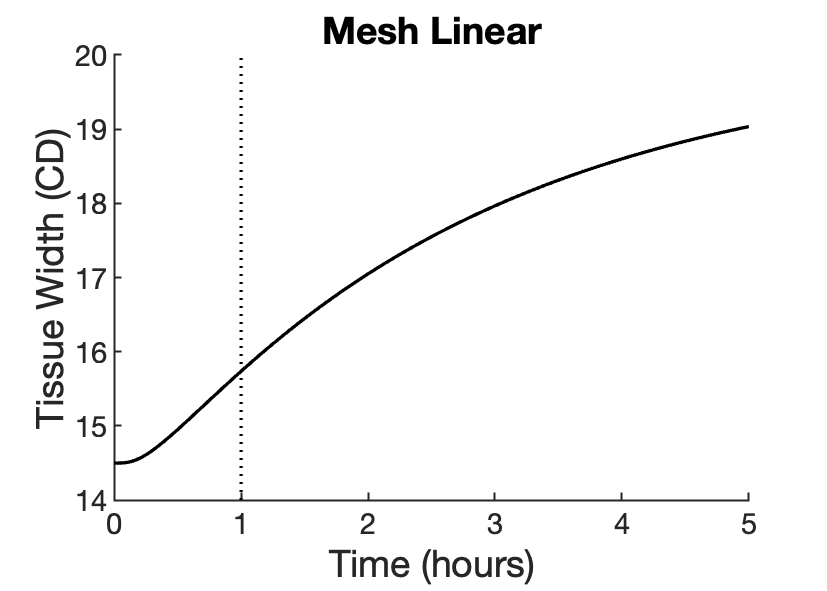
\includegraphics[width=4.9cm, trim={0.0cm 0.0cm 0.0cm 0.0cm}, clip]{Figs/Test02aMonolayerGrowth1dChainHeterogeneousChainMesh_LinearWidth}
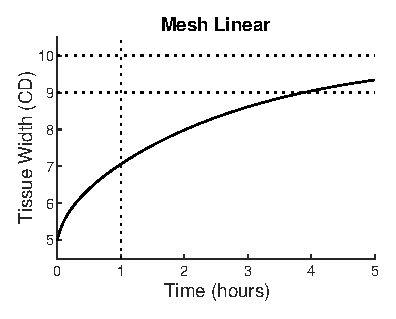
\includegraphics[width=4.9cm, trim={0.0cm 0.0cm 0.0cm 0.0cm}, clip]{Figs/Test02aMonolayerGrowth1dChainHeterogeneousChainMesh_LinearInnerWidth}
\end{center}\
\vspace{-0.5cm}
\caption{{\bf VT Heterogeneous.} 
	TODO. }
\label{fig:todo}
\end{figure}

%%%%%%% Figure %%%%%%%%
\begin{figure}[h]
%
\vspace{-0.5cm}
\begin{center}
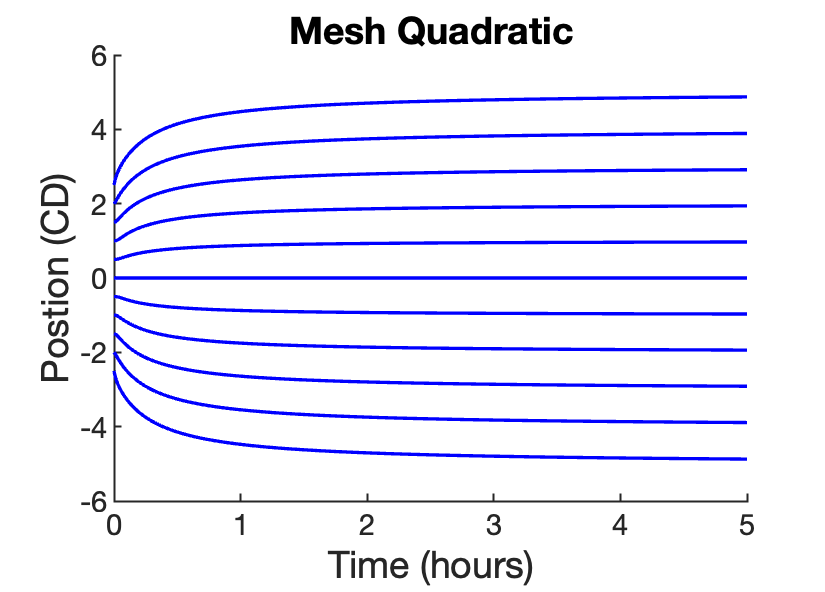
\includegraphics[width=4.9cm, trim={0.0cm 0.0cm 0.0cm 0.0cm}, clip]{Figs/Test02aMonolayerGrowth1dChainHomogeneousChainMesh_Quadratic.png}
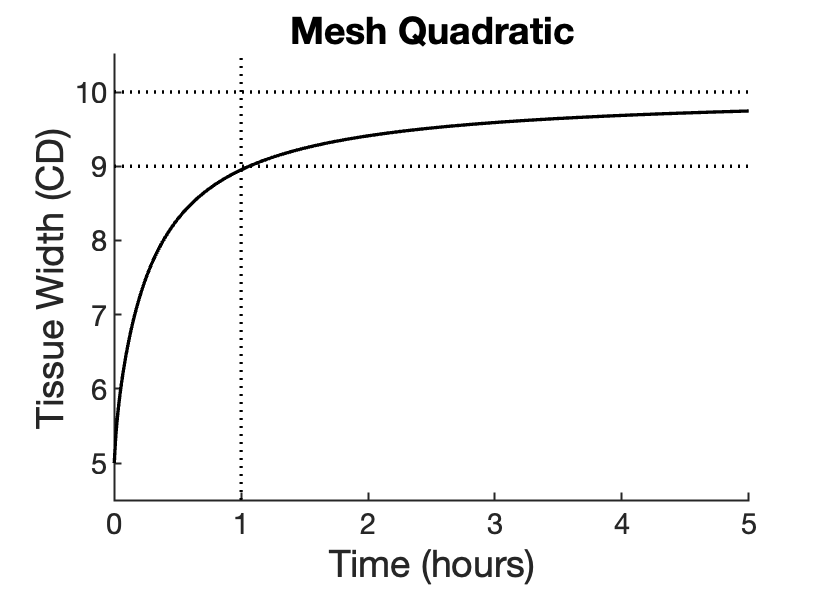
\includegraphics[width=4.9cm, trim={0.0cm 0.0cm 0.0cm 0.0cm}, clip]{Figs/Test02aMonolayerGrowth1dChainHomogeneousChainMesh_QuadraticWidth}
\end{center}
\vspace{-0.5cm}
\caption{{\bf VT homogeneous.} 
	TODO. }
\label{fig:todo}
\end{figure}

%%%%%%% Figure %%%%%%%%
\begin{figure}[h]
%
\begin{center}
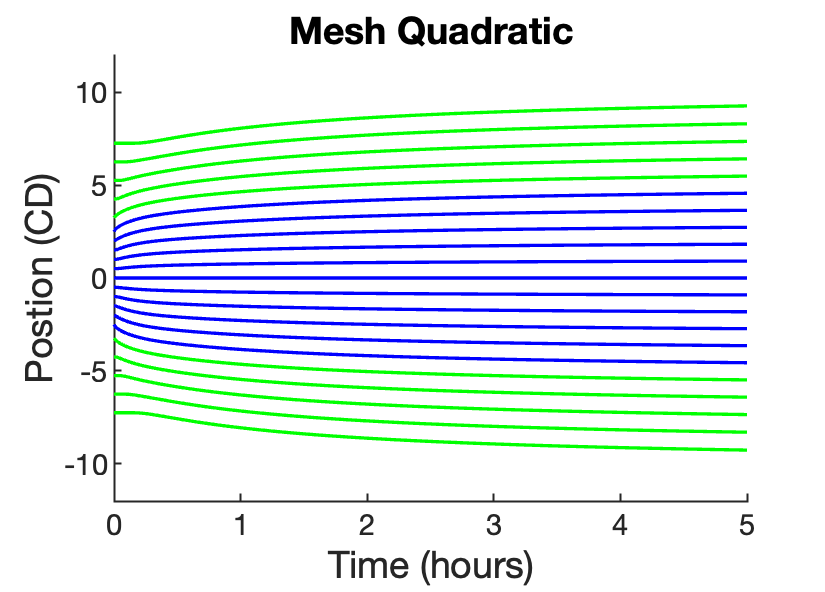
\includegraphics[width=4.9cm, trim={0.0cm 0.0cm 0.0cm 0.0cm}, clip]{Figs/Test02aMonolayerGrowth1dChainHeterogeneousChainMesh_Quadratic.png}
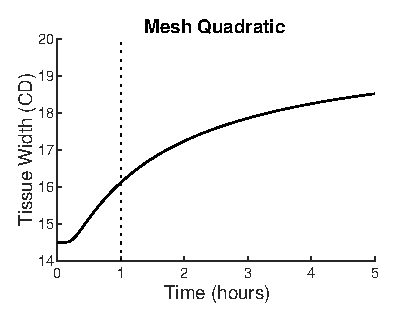
\includegraphics[width=4.9cm, trim={0.0cm 0.0cm 0.0cm 0.0cm}, clip]{Figs/Test02aMonolayerGrowth1dChainHeterogeneousChainMesh_QuadraticWidth}
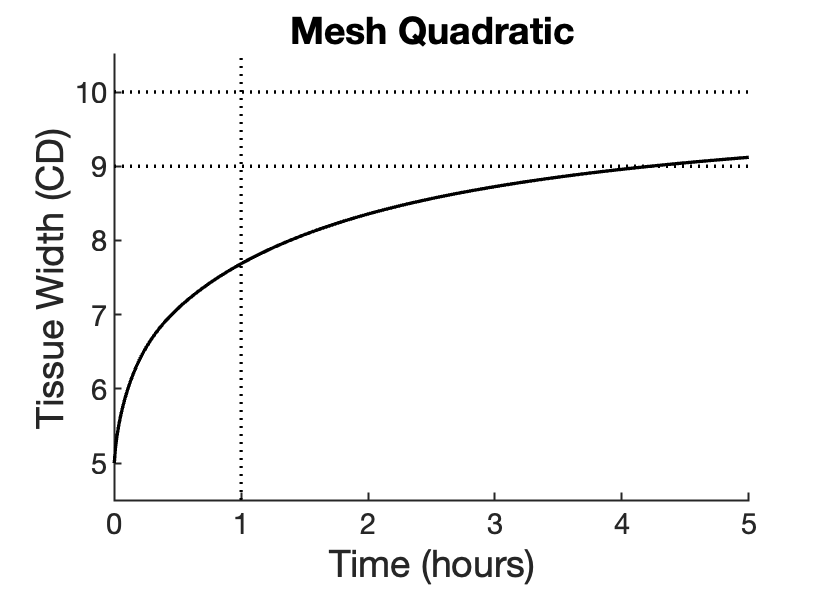
\includegraphics[width=4.9cm, trim={0.0cm 0.0cm 0.0cm 0.0cm}, clip]{Figs/Test02aMonolayerGrowth1dChainHeterogeneousChainMesh_QuadraticInnerWidth}
\end{center}\
\vspace{-0.5cm}
\caption{{\bf VT Heterogeneous.} 
	TODO. }
\label{fig:todo}
\end{figure}

%%%%%%% Figure %%%%%%%%
\begin{figure}[h]
%
\begin{center}
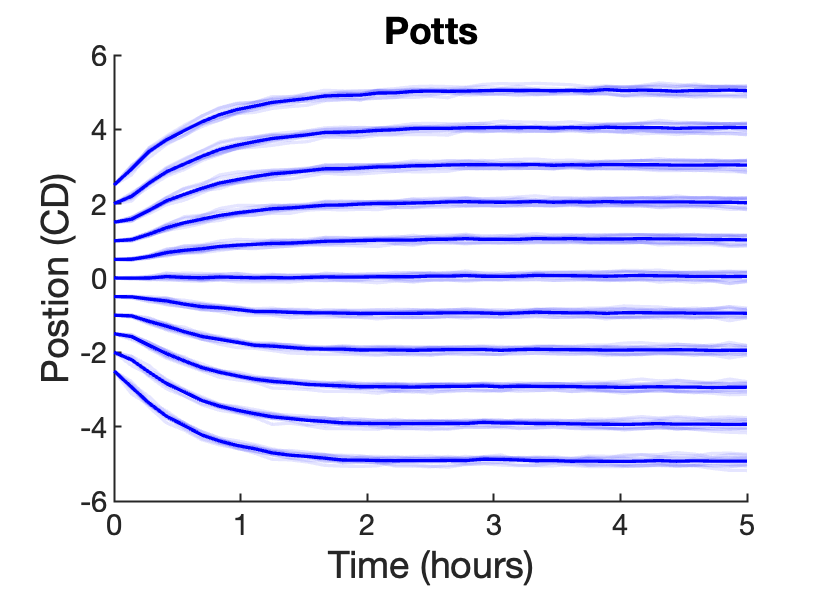
\includegraphics[width=4.9cm, trim={0.0cm 0.0cm 0.0cm 0.0cm}, clip]{Figs/Test02aMonolayerGrowth1dChainHomogeneousChainPotts.png}
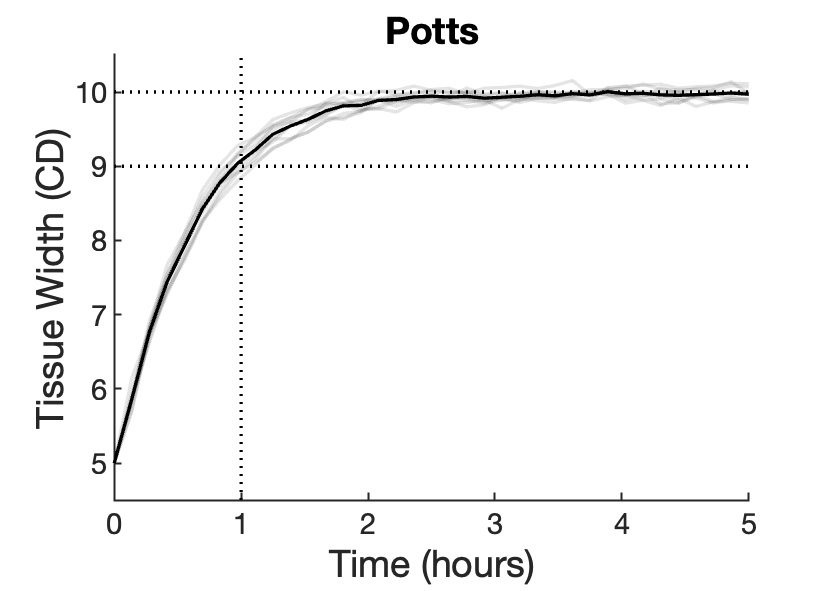
\includegraphics[width=4.9cm, trim={0.0cm 0.0cm 0.0cm 0.0cm}, clip]{Figs/Test02aMonolayerGrowth1dChainHomogeneousChainPottsWidth}
\end{center}
\vspace{-0.5cm}
\caption{{\bf CPM Homogeneous.} 
	TODO. }
\label{fig:todo}
\end{figure}

%%%%%%% Figure %%%%%%%%
\begin{figure}[h!]
%
\begin{center}
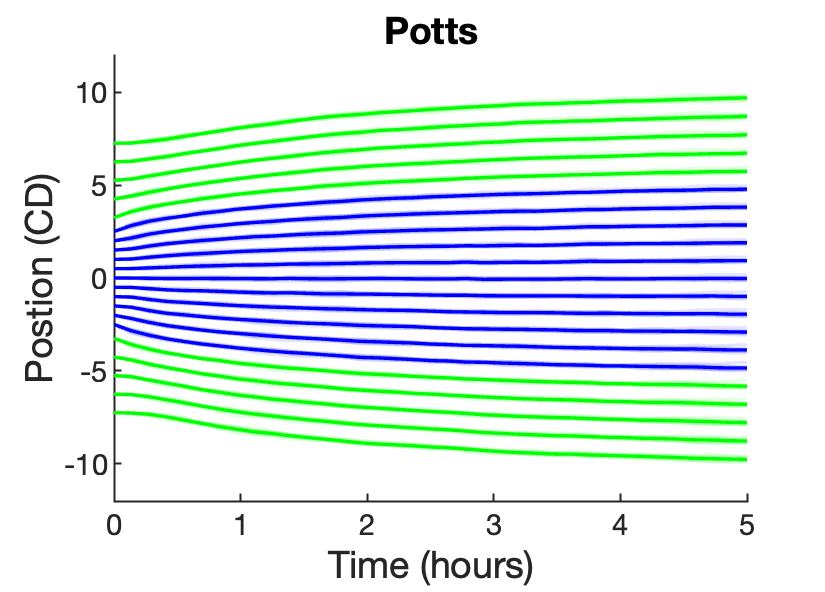
\includegraphics[width=4.9cm, trim={0.0cm 0.0cm 0.0cm 0.0cm}, clip]{Figs/Test02aMonolayerGrowth1dChainHeterogeneousChainPotts.png}
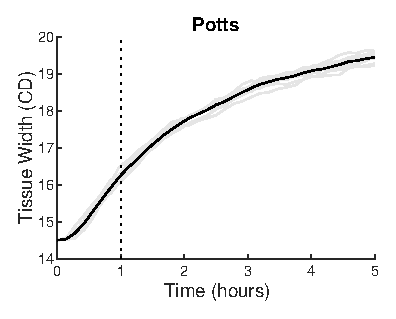
\includegraphics[width=4.9cm, trim={0.0cm 0.0cm 0.0cm 0.0cm}, clip]{Figs/Test02aMonolayerGrowth1dChainHeterogeneousChainPottsWidth}
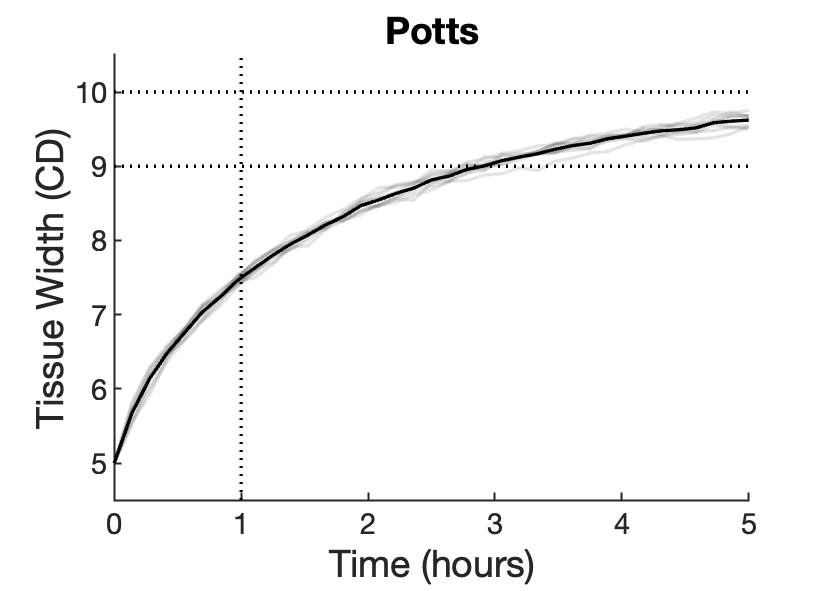
\includegraphics[width=4.9cm, trim={0.0cm 0.0cm 0.0cm 0.0cm}, clip]{Figs/Test02aMonolayerGrowth1dChainHeterogeneousChainPottsInnerWidth}
\end{center}
\vspace{-0.5cm}
\caption{{\bf CPM Heterogeneous.} 
	TODO. }
\label{fig:todo}
\end{figure}

\end{document}
